\documentclass[11pt,a4paper]{article}

% ── Packages ──
\pdfminorversion=7
\usepackage[top=0.9in,left=0.9in,right=0.9in,bottom=1.2in]{geometry}
\usepackage{array}
\usepackage{ragged2e}
\usepackage{setspace}
\usepackage{hyperref}
\usepackage{enumitem}
\usepackage{graphicx}
\usepackage{eso-pic}
\usepackage{fancyhdr}
\usepackage{tabularx}
\usepackage{float}
\usepackage{xcolor}
\usepackage{parskip}
\usepackage{colortbl}
\usepackage{longtable}
\usepackage{caption}
\usepackage{bookmark}
\usepackage{titlesec}

% ── Font (Helvetica / Arial-like, matching SRS) ──
\usepackage[T1]{fontenc}
\usepackage[scaled=0.95]{helvet}
\renewcommand{\familydefault}{\sfdefault}
\setstretch{1.0}
\frenchspacing

% ── Colours (matching SRS) ──
\definecolor{tableheader}{RGB}{240, 240, 240}
\definecolor{tablerow}{RGB}{250, 250, 250}

% ── Hyperref setup ──
\hypersetup{
    colorlinks=true,
    linkcolor=blue,
    urlcolor=blue,
    citecolor=blue,
    pdfauthor={Paragon Assurance},
    pdftitle={QA Validating Report -- PA-QAR-2026-001},
}

% ── Change Figure captions to Annex ──
\renewcommand{\figurename}{Annex}

% ── Compact spacing ──
\setlength{\parskip}{0.4em}
\setlist{nosep, leftmargin=1.5em}
\titlespacing*{\section}{0pt}{1em}{0.4em}
\titlespacing*{\subsection}{0pt}{0.8em}{0.3em}
\titlespacing*{\subsubsection}{0pt}{0.6em}{0.2em}

% ── Global table row height ──
\renewcommand{\arraystretch}{1.4}

% ── Header/Footer ──
\pagestyle{fancy}
\fancyhf{}
\lhead{\textbf{Paragon Assurance}}
\rhead{QA Validating Report (PA-QAR-2026-001)}
\cfoot{\thepage}
\renewcommand{\headrulewidth}{0.4pt}
\setlength{\headheight}{20pt}

% ── Column type for wrapped text ──
\newcolumntype{L}[1]{>{\RaggedRight\arraybackslash}p{#1}}

% ── Document ──
\begin{document}

% ══════════════════════════════════════════════════════════════
% Cover Page
% ══════════════════════════════════════════════════════════════
\thispagestyle{empty}
\fancyhf{}
\lhead{}
\rhead{}
\cfoot{}
\renewcommand{\headrulewidth}{0pt}

\newgeometry{top=4.5cm,left=0.9in,right=0.9in,bottom=1.2in}

% ── Letterhead for cover page only ──
\AddToShipoutPictureBG*{%
  \AtPageLowerLeft{%
    
\includegraphics[width=\paperwidth,height=\paperheight]{Paragon_Letterhead.pdf}%
  }%
}

\begin{center}

\includegraphics[width=0.45\textwidth]{paragon_assurance_logo.jpg}\\[0.8cm]

\LARGE\textbf{Quality Assurance Validating Report}\\[0.4cm]
\large\textbf{Requirements Engineering Process ---\\Biometric Student Attendance System}\\[0.8cm]

\textbf{\Large Paragon Assurance}\\[0.2cm]
19 March 2026
\end{center}

\vspace{0.8cm}

\begin{table}[H]
\centering\small
\begin{tabular}{|>{\raggedright\arraybackslash}m{0.22\textwidth}|>{\raggedright\arraybackslash}m{0.22\textwidth}|>{\raggedright\arraybackslash}m{0.22\textwidth}|>{\raggedright\arraybackslash}m{0.22\textwidth}|}
\hline
\rowcolor{tableheader}
\textbf{Document ID} & \textbf{Version} & \textbf{Audit Period} & \textbf{Submitted to} \\\hline
PA-QAR-2026-001 & 1.0 & 15--19 March 2026 & Nevon Solutions (Team P2-1561W) \\\hline
\end{tabular}
\end{table}

\begin{table}[H]
\centering\small
\begin{tabular}{|>{\raggedright\arraybackslash}m{0.44\textwidth}|>{\raggedright\arraybackslash}m{0.44\textwidth}|}
\hline
\rowcolor{tableheader}
\textbf{QA Auditor} & \textbf{Role} \\\hline
Chng Zong Han & QA Auditor \\\hline
\end{tabular}
\end{table}

\restoregeometry
\newpage

% Restore standard headers
\pagestyle{fancy}
\fancyhf{}
\lhead{\textbf{Paragon Assurance}}
\rhead{QA Validating Report (PA-QAR-2026-001)}
\cfoot{\thepage}
\renewcommand{\headrulewidth}{0.4pt}
\setlength{\headheight}{20pt}

% ══════════════════════════════════════════════════════════════
% Table of Contents
% ══════════════════════════════════════════════════════════════
\tableofcontents
\newpage

% ══════════════════════════════════════════════════════════════
% 1. Executive Summary
% ══════════════════════════════════════════════════════════════
\section{Executive Summary}

\subsection{Audit Context}

Paragon Assurance was engaged by BioSec Educational Institution as an independent external Quality Assurance (QA) vendor to audit the Requirements Engineering (RE) process conducted by Nevon Solutions (Team P2-1561W) for the Biometric Student Attendance System. The audit scope covers three RE methods --- Analysing, Specifying, and Validating --- in accordance with the QA auditor's mandate. The Eliciting method is excluded, as it was conducted by BioSec prior to vendor engagement and falls outside the QA audit boundary. The audit additionally evaluates the Validating method's QC component by assessing whether the assigned QC team (Veridion Labs) followed a compliant audit process.

The principal process artefacts reviewed are: Analysing Report (NS-AR-2026-001, v1.0), Software Requirements Specification (NS-SRS-2026-001, v0.8), Project Specification (BS-PS-2026-001, v1.0), Requirements repository (GitHub), QC Audit Report (Veridion Labs), and Clarification session records BC-01 (07/02/2026) and TC-02 (09/02/2026).

\subsection{Summary of Findings}

The audit identified \textbf{six (6) process non-compliance instances} across the three RE methods audited. No corrective actions or remediation steps are prescribed; findings are presented to Nevon Solutions for review and decision.

\begin{table}[H]
\centering\small
\begin{tabular}{|l|c|>{\RaggedRight\arraybackslash}m{8cm}|}
\hline
\rowcolor{tableheader}
\textbf{Severity} & \textbf{Count} & \textbf{Error IDs} \\\hline
Critical        & 1 & PA-ERR-002 (SRS Sign-off Absent --- Validating Method Incomplete) \\\hline
High            & 1 & PA-ERR-001 (Open Issues Unresolved) \\\hline
High-to-Medium  & 3 & PA-ERR-003 (2FA Contradiction), PA-ERR-004 (Enrolment Not Elicited), PA-ERR-005 (Terminology Inconsistency) \\\hline
Medium          & 1 & PA-ERR-006 (SRS Below Version 1.0) \\\hline
\end{tabular}
\caption{Summary of findings by severity}
\end{table}

Key non-compliance areas:

\begin{itemize}
    \item \textbf{The SRS has no customer or vendor signatures anywhere in the document.} All four designated approver fields in SRS \S9 are blank. The Validating method requires formal SRS authorisation before external audit release; this step was not completed (PA-ERR-002).
    \item Three open issues from the Analysing phase remain unresolved in the submitted SRS despite a stated resolution deadline of 20 February 2026 (PA-ERR-001).
    \item A contradictory 2FA scope specification was not resolved during the Clarify phase (PA-ERR-003).
    \item The biometric student enrolment process --- a prerequisite for all scan-based functions --- was not elicited and is absent from the SRS (PA-ERR-004).
    \item Attendance status terminology is inconsistent across SRS sections and the Data Dictionary (PA-ERR-005).
    \item The SRS was submitted at Version 0.8, below the Version 1.0 threshold expected for external audit release (PA-ERR-006).
\end{itemize}

The QC team (Veridion Labs) is assessed as process-compliant: a documented plan with 10 inspection techniques, a self-contained checklist of 21 items, findings covering all three required error types (Authorship, Omission, Contradiction), and a complete sign-off by all four team members. A detailed QA audit of the QC Validating process is presented in Section~\ref{sec:qc-audit}.

% ══════════════════════════════════════════════════════════════
% 2. QA Plan
% ══════════════════════════════════════════════════════════════
\section{QA Plan}

\subsection{Target Process Description}

The process under audit is the Requirements Engineering (RE) process as performed by Nevon Solutions for the Biometric Student Attendance System, Customer BioSec Educational Institution, Project Reference P2-1561W. QA audits the \emph{process} that produces the work product, not the work product itself. The error type for all QA findings is \textbf{Process Non-Compliance} --- an instance where the RE process deviated from defined process requirements through omission, incorrect execution, or unauthorised deviation.

The RE process under audit comprises three sequential methods:

\textbf{Analysing Method} --- receiving the BioSec Project Specification, assessing requirements for congruency using the IRC, resolving incongruities through BCIC process (Breakdown, Clarify, Interpret, Categorise), and producing a regulated-revision requirements repository. Phases audited: Breakdown (IRC application, decomposition), Clarify (BC-01 and TC-02 sessions, open issue management), Carrying forward (PS model revision), and Codification.

\textbf{Specifying Method} --- interpreting, categorising, and specifying the analysed requirements into the SRS document (NS-SRS-2026-001). Phases audited: Interpret and Categorise, Specify (SRS drafting, template application), iRTM (standalone file, chain-of-custody), and Change mitigation.

\textbf{Validating Method} --- applying quality control measures onto the SRS and conducting quality assurance audit. Components: Customer/Vendor validation (SRS sign-off, editorial checks) and QC audit process (plan, checklist, execution, findings preservation).

\subsection{Context and Goals}

\textbf{Context:} The BioSec project involves developing a cloud-hosted Biometric Student Attendance Management System to replace manual paper-based processes across five campuses in Singapore. The system handles biometric fingerprint data from minors and must comply with Singapore's PDPA. All artefacts were reviewed under a desktop review model.

\textbf{Goals:} (1) Determine whether the Analysing method was applied in full; (2) Determine whether the Specifying method complies with process requirements; (3) Determine whether the Validating method was completed; (4) Identify all instances of process non-compliance with evidence sufficient for review and decision.

\subsection{Work Breakdown}

The audit was structured in five phases conducted by a single QA auditor ({\raise.17ex\hbox{$\scriptstyle\sim$}}8 hours total): Preparation (2h), Evidence Collection (2h), Process Verification (2h), Observation Recording (1h), and Reporting (1h). See Appendix~\ref{app:timeline} for the detailed timeline.

% ══════════════════════════════════════════════════════════════
% 3. QA Checklist
% ══════════════════════════════════════════════════════════════
\section{QA Checklist}

The checklist addresses process compliance across four domains using three investigation methods: \textbf{M1} (Artefact Inspection), \textbf{M2} (Traceability and Cross-Reference), and \textbf{M3} (Declaration and Sign-Off Review). Rating key: S = Satisfied, PS = Partially Satisfied, NS = Not Satisfied, N/A = Not Applicable. Full checklist with detailed notes is in Appendix~\ref{app:checklist}.

\begin{longtable}{|L{0.8cm}|>{\RaggedRight\arraybackslash}m{9cm}|L{1.3cm}|L{1.3cm}|}
\caption{QA checklist summary (see Appendix~\ref{app:checklist} for full notes)}\\
\hline
\rowcolor{tableheader}
\textbf{ID} & \textbf{Checklist Item} & \textbf{Method} & \textbf{Rating} \\\hline
\endhead
\multicolumn{4}{|l|}{\cellcolor{tableheader}\textbf{Domain A --- Analysing Method}} \\\hline
A.1 & PS copy in repository & M1 & S \\\hline
A.2 & All PS requirements subjected to IRC analysis & M1 & S \\\hline
A.3 & Ambiguous requirements quantified during Clarify & M1, M2 & PS \\\hline
A.4 & Clarification sessions with all stakeholder groups & M1 & S \\\hline
A.5 & Meeting minutes formally recorded & M1 & S \\\hline
A.6 & Compound requirements decomposed & M1, M2 & S \\\hline
A.7 & Open issues documented with deadlines & M1 & PS \\\hline
A.8 & PS models carried forward & M1, M2 & S \\\hline
A.9 & PS models revised during Analysis & M1, M2 & S \\\hline
A.10 & IRC exists as standalone document & M1 & S \\\hline
A.11 & IRC was actually used & M1 & S \\\hline
A.12 & Plan for Analysing phase & M1 & S \\\hline
A.13 & PS items codified in repository & M1, M2 & S \\\hline
A.14 & Biometric enrolment process elicited & M1, M2 & NS \\\hline
\multicolumn{4}{|l|}{\cellcolor{tableheader}\textbf{Domain B --- Specifying Method}} \\\hline
B.1 & SRS references recognised template & M1 & S \\\hline
B.2 & Requirements traceable via iRTM & M1, M2 & PS \\\hline
B.3 & iRTM exists as standalone file & M1 & S \\\hline
B.4 & Terminology consistent across SRS & M2 & NS \\\hline
B.5 & Open issues resolved before SRS finalisation & M1, M2 & NS \\\hline
B.6 & Contradictions resolved before Specifying & M2 & NS \\\hline
B.7 & New model source files present & M1 & N/A \\\hline
B.8 & Change Mitigation template exists & M1 & S \\\hline
B.9 & SRS at final ($\geq$ v1.0) version & M1 & NS \\\hline
\multicolumn{4}{|l|}{\cellcolor{tableheader}\textbf{Domain C --- Validating Method}} \\\hline
C.1 & SRS formally signed off & M3 & NS \\\hline
C.2 & Spell check evidence & M3 & PS \\\hline
C.3 & Grammar check evidence & M3 & PS \\\hline
C.4 & Editorial review evidence & M3 & NS \\\hline
C.5 & QC team has documented audit plan & M1 & S \\\hline
C.6 & QC team has structured checklist & M1 & S \\\hline
C.7 & QC team documented findings with evidence & M1 & S \\\hline
C.8 & QC findings in retrievable format & M1 & S \\\hline
\multicolumn{4}{|l|}{\cellcolor{tableheader}\textbf{Domain D --- Process Artefact Integrity}} \\\hline
D.1 & All required artefacts present & M1 & S \\\hline
D.2 & Artefacts internally consistent & M2 & PS \\\hline
D.3 & AI and Plagiarism declarations present & M1, M3 & S \\\hline
D.4 & Repository structured correctly & M1 & S \\\hline
D.5 & Change Mitigation Strategies documented & M1 & S \\\hline
D.6 & Risk Analysis present & M1 & S \\\hline
D.7 & Version control and metadata complete & M1 & PS \\\hline
\end{longtable}

% ══════════════════════════════════════════════════════════════
% 4. QA Error Detection
% ══════════════════════════════════════════════════════════════
\section{QA Error Detection}

All findings are of error type \textbf{Process Non-Compliance}.

\begin{table}[H]
\centering\small
\begin{tabular}{|L{1.8cm}|L{3cm}|>{\RaggedRight\arraybackslash}m{7.5cm}|}
\hline
\rowcolor{tableheader}
\textbf{Error ID} & \textbf{Location} & \textbf{Characteristic} \\\hline
PA-ERR-001 & AR \S3.5; SRS \S2.5, \S3.3, \S6.5 & Three open issues remain unresolved 11+ days past the RPO/RTO deadline of 20/02/2026. \\\hline
PA-ERR-002 & SRS \S9; full repository & All four sign-off fields blank. No supplementary authorisation evidence found. Validating method not completed. \\\hline
PA-ERR-003 & SRS \S3.1 UR-MOB-06; \S5.3 NFR-SEC-03 & 2FA required for parents/teachers in UR-MOB-06 but restricted to administrators in NFR-SEC-03. Not resolved during Clarify. \\\hline
PA-ERR-004 & SRS \S4; AR \S3.3--3.4; repository & Biometric enrolment --- prerequisite for scan-based operations --- not elicited. No requirement exists despite BOR-0-03 referencing it. \\\hline
PA-ERR-005 & SRS \S3.1, \S4.3.2; Data Dictionary C.4 & Three-way terminology inconsistency: ``Attended'' vs ``Excused, Attended...'' vs ``Present.'' \\\hline
PA-ERR-006 & SRS cover; AR cover & SRS at v0.8 (03/03/2026); AR released at v1.0 (08/02/2026). SRS handed over before completion. \\\hline
\end{tabular}
\caption{Error detection register}
\end{table}

% ══════════════════════════════════════════════════════════════
% 5. QA Findings
% ══════════════════════════════════════════════════════════════
\section{QA Findings}
\label{sec:findings}

Each finding presents a CRaM analysis of the non-compliance instance. Findings are presented without corrective action; Nevon Solutions is to determine remediation at its discretion. Full evidence tables are in Appendix~\ref{app:findings}.

\subsection{PA-FND-001 --- Open Issues Unresolved at SRS Finalisation}

\noindent\textbf{Evidence:} See \ref{ann:evidence-001} (Annex)

\noindent\textbf{Error:} PA-ERR-001 \quad \textbf{Severity:} High \quad \textbf{Phase:} Analysing --- Open Issue Management; Specifying --- SRS Finalisation

The Analysing Report \S3.5 documents three open issues: MCS Integration Security (no deadline), Disaster Recovery RPO/RTO (deadline 20/02/2026), and Biometric Template Storage Format. The SRS dated 03/03/2026 retains all three as unresolved (\S2.5, \S3.3, \S6.5 NFR-DOC-03). The RPO/RTO deadline passed without resolution and no formal deferral was presented. This constitutes a failure of the open issue resolution protocol required before SRS release.

\subsection{PA-FND-002 --- SRS Sign-off Entirely Absent --- Validating Method Incomplete}

\noindent\textbf{Evidence:} See \ref{ann:evidence-002} (Annex)

\noindent\textbf{Error:} PA-ERR-002 \quad \textbf{Severity:} Critical \quad \textbf{Phase:} Validating --- Customer SRS Authorisation

SRS \S9 provides sign-off fields for four designated roles; all four rows are entirely blank. The QA auditor conducted a full repository inspection: no signed declaration, no BioSec confirmation document, no interview record, and no alternative authorisation evidence of any kind was found. The Analysing Report sign-off is correctly completed (Loh Wen Xuan, 13/02/2026), confirming the team knows the protocol. The SRS sign-off is the terminal step of the Validating method; its absence means the method was not completed and the SRS was released as an unauthorised draft.

\subsection{PA-FND-003 --- 2FA Scope Contradiction Not Resolved}

\noindent\textbf{Evidence:} See \ref{ann:evidence-003} (Annex)

\noindent\textbf{Error:} PA-ERR-003 \quad \textbf{Severity:} High-to-Medium \quad \textbf{Phase:} Analysing --- Clarify; Specifying --- Cross-Section Review

UR-MOB-06 mandates 2FA for parents and teachers (mobile), while NFR-SEC-03 mandates 2FA exclusively for administrators (web portal). These are directly contradictory. BC-01 and TC-02 session outcomes contain no reference to 2FA scope resolution.

\subsection{PA-FND-004 --- Biometric Student Enrolment Process Not Elicited}

\noindent\textbf{Error:} PA-ERR-004 \quad \textbf{Severity:} High-to-Medium \quad \textbf{Phase:} Analysing --- Breakdown and Clarify

Biometric enrolment --- the process of capturing and registering a student's fingerprint template --- is a logical prerequisite for all scan-based operations. No enrolment requirement exists in the SRS (\S4), the repository, or the Analysing Report session outcomes. However, BOR-0-03 acceptance criteria reference ``biometric enrolment,'' confirming the team was aware of the concept but did not elicit it.

\subsection{PA-FND-005 --- Attendance Status Terminology Inconsistency}

\noindent\textbf{Error:} PA-ERR-005 \quad \textbf{Severity:} High-to-Medium \quad \textbf{Phase:} Specifying --- Cross-Section Consistency Review

Three-way inconsistency: UR-MOB-01 uses ``Attended, Absent, Late, or Excused''; \S4.3.2 uses ``Excused, Attended, Late, Absent''; Data Dictionary Table C.4 uses ``Present.'' This should have been detected and unified during the Specifying phase.

\subsection{PA-FND-006 --- SRS Submitted Below Final Version Threshold}

\noindent\textbf{Evidence:} See \ref{ann:evidence-006} (Annex)

\noindent\textbf{Error:} PA-ERR-006 \quad \textbf{Severity:} Medium \quad \textbf{Phase:} Specifying --- Version Control and Release Protocol

The SRS bears Version 0.8 (03/03/2026) while the Analysing Report was released at Version 1.0 (08/02/2026). Sub-1.0 version numbers indicate draft status. This is corroborated by incomplete sign-off (PA-FND-002) and unresolved open issues (PA-FND-001).

% ══════════════════════════════════════════════════════════════
% 6. QA Audit of QC Validating Process
% ══════════════════════════════════════════════════════════════
\section{QA Audit of QC Validating Process}
\label{sec:qc-audit}

This section assesses the QC audit process conducted by Veridion Labs on the SRS. The QA auditor assesses the \emph{process} of the QC audit, not the correctness of individual QC findings. Detailed sub-assessments are in Appendix~\ref{app:qc-detail}.

\textbf{QC Team:} Muhammad Ridwan Putra Jasni (QC Audit Lead), Lin Yuhao, Muhammad Mikhail Bin Mazlan, and Kannan s/o Rajamohan (QC Specialists).

The QC audit is assessed as \textbf{process-compliant}:

\begin{enumerate}
    \item \textbf{Plan:} Documented plan with target workproduct, context, goals, 10 inspection techniques (exceeding the minimum of six), role-based work breakdown (4 members), and indicative 4-stage timeline ({\raise.17ex\hbox{$\scriptstyle\sim$}}6 hours).
    \item \textbf{Checklist:} Self-contained checklist of 21 items (QC1--QC21) across 7 SRS sections, with CRaM-specific items tailored to the Biometric Student Attendance System.
    \item \textbf{Error Detection:} 12 error instances across all three required types: Contradiction (3), Omission (5), Authorship (4).
    \item \textbf{Findings:} 12 findings with Context-Result-Analysis structure and severity classifications (High: 5, Medium: 4, Low: 3).
    \item \textbf{Reporting:} Retrievable PDF report with structured appendices, cross-referenced error detection, and findings summary.
    \item \textbf{Sign-off:} All four team members signed.
\end{enumerate}

\textbf{No QC process non-compliance was identified.}

% ══════════════════════════════════════════════════════════════
% 7. Sign-Off
% ══════════════════════════════════════════════════════════════
\section{Sign-Off}

This QA Validating Report (PA-QAR-2026-001, Version 1.0) is formally submitted to Nevon Solutions (Team P2-1561W) by Paragon Assurance. The six (6) process non-compliance findings documented in Sections 4 and 5, together with the QC process audit in Section 6, represent the complete output of the QA audit of Nevon Solutions' Requirements Engineering process for the Biometric Student Attendance System (Project P2-1561W).

The QC audit conducted by Veridion Labs is assessed as process-compliant (Section~\ref{sec:qc-audit}). No QC process non-compliance was identified.

No modifications to any Nevon Solutions process artefact have been made by the QA auditor. No corrective actions or remediation steps are prescribed. This report documents findings only; Nevon Solutions is to determine appropriate action at its discretion.

\vspace{0.8cm}

\begin{table}[h!]
\centering
\begin{tabular}{|l|l|l|l|}
\hline
\rowcolor{tableheader}
\textbf{Role} & \textbf{Name} & \textbf{Signature} & \textbf{Date} \\\hline
QA Auditor & Zong Han & 
\includegraphics[width=3.5cm,height=0.8cm]{../Brigman/Signatures/signature_zonghan.jpg} & 19/03/2026 \\\hline
\end{tabular}
\end{table}

\newpage

% ══════════════════════════════════════════════════════════════
%  APPENDICES
% ══════════════════════════════════════════════════════════════
\appendix

\part*{Appendices}
\phantomsection
\addcontentsline{toc}{part}{Appendices}

% ── Appendix page numbering: A-1, A-2, B-1, etc. ──
\newcommand{\appendixprefix}{A}
\renewcommand{\thepage}{\appendixprefix-\arabic{page}}

% ── Appendix A: Full QA Checklist ──
\renewcommand{\appendixprefix}{A}
\setcounter{page}{1}
\section{Full QA Checklist}
\label{app:checklist}

\subsection{Domain A --- Analysing Method}

\begin{longtable}{|L{0.8cm}|L{4cm}|L{1.3cm}|L{1.3cm}|L{5.5cm}|}
\hline
\rowcolor{tableheader}
\textbf{ID} & \textbf{Checklist Item} & \textbf{Method} & \textbf{Rating} & \textbf{Notes} \\
\hline
\endhead
A.1 & Does the vendor have a copy of the Project Specification (PS) in their repository? & M1 & S & Project Specification\_1561W.pdf present in repository root. \\\hline
A.2 & Were all PS requirements subjected to the Breakdown/IRC analysis (congruency check)? & M1 & S & Analysing Report \S2.1--2.2 documents full IRC application across all PS requirements. Five incongruity categories assessed. \\\hline
A.3 & Were all ambiguous requirements quantified during the Clarify phase? & M1, M2 & PS & Most ambiguous requirements were resolved (BC-01 outcomes). BOR-1-MOB-01 still references ``institutional policies'' without specific policy documents (flagged; resolution pending). \\\hline
A.4 & Were clarification sessions conducted with all relevant stakeholder groups? & M1 & S & BC-01 (07/02/2026): BioSec Academic Administrator, Parent Representative, Campus Operations Manager, Account Manager. TC-02 (09/02/2026): BioSec IT Manager, Network Infrastructure Lead. Both documented in AR \S3.3--3.4. \\\hline
A.5 & Were meeting minutes formally recorded with attendees, focus, and outcomes? & M1 & S & BC-01 and TC-02 documented in AR \S3.3--3.4 with attendees, clarification focus, and key outcomes. \\\hline
A.6 & Were all compound requirements decomposed into atomic requirements? & M1, M2 & S & AR \S2.2--2.3 documents decomposition of BOR-1-MOB-02, BOR-1-MOB-03, BOR-1-WEB-01, BOR-1-WEB-02, TR-1-BE-01, and TR-1-BE-05 into atomic requirements with traceability. \\\hline
A.7 & Were open issues formally documented with resolution deadlines? & M1 & PS & AR \S3.5 documents three open issues with stated deadlines and assigned parties. However, the RPO/RTO deadline of 20/02/2026 was not met prior to SRS finalisation (see PA-ERR-001). \\\hline
A.8 & Were models from the PS carried forward into the Analysis phase? & M1, M2 & S & paper-napkin-model.jpg (original from PS) and context-diagram.pdf (revised) both present in repository requirement-models/. \\\hline
A.9 & Is there proof that the PS models were revised during Analysis? & M1, M2 & S & context-diagram.pdf is a revised version reflecting TC-02 outcomes with six external entities. Original PS model retained separately. Data Dictionary revised with three new tables (C.7--C.9). \\\hline
A.10 & Does the IRC exist as a standalone, usable document? & M1 & S & IRC\_Nevon\_Solutions.pdf is a standalone checklist-format document with 9 categories. Extractable and distributable. \\\hline
A.11 & Is there evidence that the IRC was actually used (not merely created)? & M1 & S & IRC document contains 9 completed categories with project-specific findings tied to PS requirements. Not a blank template. \\\hline
A.12 & Did the vendor have a plan for the Analysing phase? & M1 & S & BioSec Gantt Chart.xlsx documents structured sessions BC-01 and TC-02 with assigned dates and deliverables. \\\hline
A.13 & Were items from the PS properly codified in the repository? & M1, M2 & S & bizops-requirements.md and technical-requirements.md carry a consistent BOR/TR identifier scheme. All requirements codified with unique IDs. \\\hline
A.14 & Was the biometric enrolment process elicited as part of the Analysing phase? & M1, M2 & NS & No enrolment requirement appears in either the repository or the SRS. BC-01 and TC-02 outcomes make no reference to enrolment. See PA-ERR-004. \\\hline
\end{longtable}

\subsection{Domain B --- Specifying Method}

\begin{longtable}{|L{0.8cm}|L{4cm}|L{1.3cm}|L{1.3cm}|L{5.5cm}|}
\hline
\rowcolor{tableheader}
\textbf{ID} & \textbf{Checklist Item} & \textbf{Method} & \textbf{Rating} & \textbf{Notes} \\
\hline
\endhead
B.1 & Does the SRS reference a recognised template? & M1 & S & srs\_template-ieee.doc present in repository. SRS structure follows IEEE format. \\\hline
B.2 & Are all SRS requirements traceable to PS/repository requirements via iRTM? & M1, M2 & PS & iRTM is present in SRS Appendix D. However, the absence of enrolment requirements (PA-ERR-004) means the iRTM cannot account for this process gap. \\\hline
B.3 & Does the iRTM exist as a standalone, extractable file? & M1 & S & iRTM.docx is a standalone .docx file in the repository. Not embedded in the SRS PDF. \\\hline
B.4 & Is terminology consistent across all SRS sections and artefacts? & M2 & NS & Attendance status terminology is inconsistent across SRS sections. UR-MOB-01 uses ``Attended, Absent, Late, or Excused''; \S4.3.2 uses ``Excused, Attended, Late, Absent''; Data Dictionary Table C.4 uses ``Present.'' See PA-ERR-005. \\\hline
B.5 & Were all open issues from the Analysing phase resolved before SRS finalisation? & M1, M2 & NS & All three open issues in AR \S3.5 remain unresolved in the submitted SRS despite a stated deadline of 20/02/2026. See PA-ERR-001. \\\hline
B.6 & Were contradictory requirements identified during Clarify and resolved before Specifying? & M2 & NS & The 2FA scope contradiction between UR-MOB-06 and NFR-SEC-03 was not resolved. BC-01 outcomes make no reference to 2FA scope. See PA-ERR-003. \\\hline
B.7 & If new models were created in Specifying, are the source files present? & M1 & N/A & No new models created during Specifying phase. All models originated in Analysing and were carried forward. \\\hline
B.8 & If a Change Mitigation template is mentioned, does the template file exist? & M1 & S & Change Request Form Template.docx present in repository requirement-models/. \\\hline
B.9 & Was the SRS submitted at a final ($\geq$ Version 1.0) version? & M1 & NS & SRS bears Version 0.8. Analysing Report was released at Version 1.0. See PA-ERR-006. \\\hline
\end{longtable}

\subsection{Domain C --- Validating Method}

\subsubsection{C.I --- Customer/Vendor Validation}

\begin{longtable}{|L{0.8cm}|L{4cm}|L{1.3cm}|L{1.3cm}|L{5.5cm}|}
\hline
\rowcolor{tableheader}
\textbf{ID} & \textbf{Checklist Item} & \textbf{Method} & \textbf{Rating} & \textbf{Notes} \\
\hline
\endhead
C.1 & Was the SRS formally signed off by designated BioSec stakeholders before external audit release? & M3 & NS & All four sign-off fields in SRS \S9 are blank. No names, signatures, or dates recorded. See PA-ERR-002. \\\hline
C.2 & Is there evidence of a spell check before SRS submission? & M3 & PS & SRS Declaration page states the document was ``reviewed, validated, and approved'' by the Project Lead, but does not record spell check as a distinct activity. No standalone checklist or log found. \\\hline
C.3 & Is there evidence of a grammar check before SRS submission? & M3 & PS & No documentary evidence of a grammar check was found. \\\hline
C.4 & Is there evidence of an editorial review before SRS submission? & M3 & NS & No editorial check record found. Terminology inconsistencies (PA-ERR-005) indicate editorial review was either not performed or was ineffective. \\\hline
\end{longtable}

\subsubsection{C.II --- QC Audit Process}

\begin{longtable}{|L{0.8cm}|L{4cm}|L{1.3cm}|L{1.3cm}|L{5.5cm}|}
\hline
\rowcolor{tableheader}
\textbf{ID} & \textbf{Checklist Item} & \textbf{Method} & \textbf{Rating} & \textbf{Notes} \\
\hline
\endhead
C.5 & Does the QC team have a documented audit plan? & M1 & S & QC Report \S3 contains a structured plan: target workproduct identified, context and goals stated, 10 inspection techniques listed, work breakdown with 4 team members. See Section~\ref{sec:qc-audit}. \\\hline
C.6 & Does the QC team have a structured checklist? & M1 & S & QC Report \S4 and Appendix B contain a self-contained checklist of 21 items (QC1--QC21) across 7 SRS sections. See Section~\ref{sec:qc-audit}. \\\hline
C.7 & Did the QC team document findings with evidence? & M1 & S & QC Report \S5--6 document 12 findings across three error types: Authorship (4), Omission (4), Contradiction (4). See Section~\ref{sec:qc-audit}. \\\hline
C.8 & Are QC findings saved in a retrievable report format? & M1 & S & QC Report submitted as a standalone PDF with structured appendices. All 4 team members signed off (\S8). See Section~\ref{sec:qc-audit}. \\\hline
\end{longtable}

\subsection{Domain D --- Process Artefact Integrity}

\begin{longtable}{|L{0.8cm}|L{4cm}|L{1.3cm}|L{1.3cm}|L{5.5cm}|}
\hline
\rowcolor{tableheader}
\textbf{ID} & \textbf{Checklist Item} & \textbf{Method} & \textbf{Rating} & \textbf{Notes} \\
\hline
\endhead
D.1 & Are all required process artefacts present? & M1 & S & All artefacts listed in SRS Table of Contents and repository README confirmed present. \\\hline
D.2 & Are process artefacts internally consistent with SRS content? & M2 & PS & Context DFD documents six external entities consistent with SRS \S2.1. However, Data Dictionary Table C.4 uses ``Present'' inconsistent with SRS \S3.1 and \S4.3.2. \\\hline
D.3 & Do all deliverables carry a Declaration of Use of AI Tools and a Declaration on Plagiarism and Originality? & M1, M3 & S & Both the Analysing Report and the SRS carry both declarations, signed by Project Lead Loh Wen Xuan. \\\hline
D.4 & Is the requirements repository structured correctly with all required fields per requirement? & M1 & S & Repository README confirms all seven fields. Sample review confirms compliance across all requirements. \\\hline
D.5 & Are Change Mitigation Strategies documented in the SRS? & M1 & S & SRS \S8 documents three strategies: Anticipatory Contingency Requirements, Open Issues, and High-Risk Change Control Process. \\\hline
D.6 & Is a Risk Analysis present in the Analysing Report? & M1 & S & Nevon Risk Analysis Matrix.docx in repository. AR \S5 documents risks with likelihood and impact ratings. \\\hline
D.7 & Are version control and document metadata complete across all deliverables? & M1 & PS & AR (v1.0) has complete metadata. SRS (v0.8) has complete metadata but is below expected release threshold (PA-ERR-006). \\\hline
\end{longtable}

% ── Appendix B: Detailed QA Findings ──
\clearpage
\renewcommand{\appendixprefix}{B}
\setcounter{page}{1}
\section{Detailed QA Findings --- Evidence Tables}
\label{app:findings}

\subsection{PA-FND-001 --- Evidence}

\begin{table}[H]
\centering\small
\begin{tabular}{|l|L{3cm}|>{\RaggedRight\arraybackslash}m{6.5cm}|}
\hline
\rowcolor{tableheader}
\textbf{Source} & \textbf{Location} & \textbf{Content} \\\hline
Analysing Report & \S3.5 & Three open issues; RPO/RTO deadline 20/02/2026 \\\hline
SRS & \S2.5 & Biometric template storage still open; kill date 15/03/2026 \\\hline
SRS & \S3.3 & MCS encryption handshake still an open issue \\\hline
SRS & \S6.5 NFR-DOC-03 & Disaster recovery RPO/RTO ``still pending BioSec approval'' \\\hline
\end{tabular}
\end{table}

\textbf{Confirmation:} The SRS date of 03/03/2026 post-dates the RPO/RTO resolution deadline of 20/02/2026. The SRS text itself acknowledges all three issues as unresolved. No resolution or deferral documentation was presented to the QA auditor.

\subsection{PA-FND-002 --- Evidence}

\begin{table}[H]
\centering\small
\begin{tabular}{|l|L{3cm}|>{\RaggedRight\arraybackslash}m{6.5cm}|}
\hline
\rowcolor{tableheader}
\textbf{Source} & \textbf{Location} & \textbf{Content} \\\hline
SRS & \S9 Sign-off & All four rows blank: Name, Signature, Date all empty \\\hline
Repository & Full file listing & No signed declaration, confirmation document, or sign-off record found \\\hline
Repository & Interview records & No record of verbal or alternative sign-off confirmation found \\\hline
Analysing Report & Declaration, p.3 & Correctly completed: Loh Wen Xuan, signature present, dated 13/02/2026 \\\hline
\end{tabular}
\end{table}

\textbf{Confirmation:} Direct inspection of SRS \S9 confirms all sign-off fields are blank. Full repository inspection confirms no supplementary authorisation evidence exists. The Analysing Report's correctly completed sign-off confirms the team is familiar with the protocol. The Validating method was not completed.

\subsection{PA-FND-003 --- Evidence}

\begin{table}[H]
\centering\small
\begin{tabular}{|l|L{3cm}|>{\RaggedRight\arraybackslash}m{6.5cm}|}
\hline
\rowcolor{tableheader}
\textbf{Source} & \textbf{Location} & \textbf{Content} \\\hline
SRS & \S3.1 UR-MOB-06 & 2FA required for parents and teachers \\\hline
SRS & \S5.3 NFR-SEC-03 & 2FA required for administrators only \\\hline
Analysing Report & \S3.3 BC-01 & No reference to 2FA scope \\\hline
Analysing Report & \S3.4 TC-02 & No reference to 2FA scope \\\hline
\end{tabular}
\end{table}

\subsection{PA-FND-004 --- Evidence}

\begin{table}[H]
\centering\small
\begin{tabular}{|l|L{3cm}|>{\RaggedRight\arraybackslash}m{6.5cm}|}
\hline
\rowcolor{tableheader}
\textbf{Source} & \textbf{Location} & \textbf{Content} \\\hline
SRS & \S4 System Features & No enrolment feature section; seven features, none covering enrolment \\\hline
Repository & bizops-requirements.md & No enrolment requirement present \\\hline
Repository & BOR-0-03 Acceptance Criteria & ``Parental consent is collected before biometric enrolment'' --- references enrolment without a corresponding requirement \\\hline
Analysing Report & \S3.3--3.4 & No enrolment process in documented outcomes \\\hline
\end{tabular}
\end{table}

\subsection{PA-FND-005 --- Evidence}

\begin{table}[H]
\centering\small
\begin{tabular}{|l|L{3cm}|>{\RaggedRight\arraybackslash}m{6.5cm}|}
\hline
\rowcolor{tableheader}
\textbf{Source} & \textbf{Location} & \textbf{Content} \\\hline
SRS & \S3.1 UR-MOB-01 & ``Attended, Absent, Late, or Excused'' \\\hline
SRS & \S4.3.2 & ``Excused, Attended, Late, Absent'' \\\hline
SRS & Data Dictionary Table C.4 & ``Present'' --- diverges from both SRS \S3.1 and \S4.3.2 \\\hline
\end{tabular}
\end{table}

\subsection{PA-FND-006 --- Evidence}

\begin{table}[H]
\centering\small
\begin{tabular}{|l|L{3cm}|>{\RaggedRight\arraybackslash}m{6.5cm}|}
\hline
\rowcolor{tableheader}
\textbf{Source} & \textbf{Location} & \textbf{Content} \\\hline
SRS & Cover page & Version 0.8, Date: 03 March 2026 \\\hline
Analysing Report & Cover page & Version 1.0, Date: 08 February 2026 \\\hline
\end{tabular}
\end{table}

% ── Appendix C: Detailed QC Process Audit ──
\clearpage
\renewcommand{\appendixprefix}{C}
\setcounter{page}{1}
\section{Detailed QC Process Audit}
\label{app:qc-detail}

\subsection{QC Plan Assessment}

The QC Report \S3 contains a documented audit plan with the following elements:

\begin{table}[H]
\centering\small
\begin{tabular}{|l|c|>{\RaggedRight\arraybackslash}m{7.5cm}|}
\hline
\rowcolor{tableheader}
\textbf{Plan Element} & \textbf{Status} & \textbf{Evidence} \\\hline
Target workproduct & Present & \S3.1: NS-SRS-2026-001, Version 0.8, prepared by Nevon Solutions for BioSec Educational Institution \\\hline
Context and goals & Present & \S3.2: Verifies SRS clarity, completeness, and internal consistency \\\hline
Inspection techniques & Present & \S3.4: 10 techniques including close document inspection, perspective-based reading, cross-section contradiction checking, codification verification, model-to-text consistency, omission mapping, scenario-based reading, assumption reading, fact-checking, and spellcheck/grammar review \\\hline
Work breakdown & Present & \S3.5/Appendix A Table A-1: Four roles --- QC Audit Lead, Requirements Reviewer, Traceability Reviewer, Editorial and Structure Reviewer \\\hline
Timeline & Present & \S3.6/Appendix A Table A-2: Four stages totalling {\raise.17ex\hbox{$\scriptstyle\sim$}}6 hours \\\hline
Reporting protocol & Present & \S3.7: Findings recorded in report; audit team does not amend the SRS \\\hline
\end{tabular}
\end{table}

\subsection{QC Checklist Assessment}

21 items (QC1--QC21) across seven SRS sections: Introduction (QC1--3), Glossary (QC4--6), Overall Description (QC7--9), Functional Requirements (QC10--12), Interface Requirements (QC13--15), Non-Functional Requirements (QC16--18), Addenda (QC19--21). Items are CRaM-specific to the Biometric Student Attendance System and directly address all three QC error families.

\subsection{QC Error Detection Assessment}

The QC team documented findings covering all required error families: Contradiction, Omission, and Authorship.

\subsection{QC Findings Assessment}

Findings were documented with Context-Result-Analysis structure and severity classifications. All findings are signed off.

\subsection{QC Sign-off and Addenda}

All four team members signed. Addenda include Glossary (10 terms), Appendix A (Plan Tables), Appendix B (Checklist), Appendix C (Error Detection), Appendix D (Findings Summary), and References (5 sources). All appendix content is correctly linked from the main report body.

% ── Appendix D: Audit Timeline and Artefacts ──
\clearpage
\renewcommand{\appendixprefix}{D}
\setcounter{page}{1}
\section{Audit Work Allocation and Timeline}
\label{app:timeline}

\subsection{Audit Timeline}

\begin{table}[H]
\centering\small
\begin{tabular}{|l|c|>{\RaggedRight\arraybackslash}m{7cm}|c|}
\hline
\rowcolor{tableheader}
\textbf{Stage} & \textbf{Date} & \textbf{Activities} & \textbf{Hours} \\\hline
Stage 1 & 15 Mar 2026 & Document collection; confirm access; prepare audit checklist & 2 \\\hline
Stage 2 & 16 Mar 2026 & Review all artefacts; apply checklist Domains A and B & 2 \\\hline
Stage 3 & 17 Mar 2026 & Apply checklist Domains C and D; request supplementary evidence; document non-compliance & 2 \\\hline
Stage 4 & 18 Mar 2026 & CRaM analysis; cross-reference QC Report; consolidate evidence & 1 \\\hline
Stage 5 & 19 Mar 2026 & Report drafting, review, and finalisation for Nevon Solutions submission & 1 \\\hline
\textbf{Total} & & & \textbf{8} \\\hline
\end{tabular}
\end{table}

\subsection{Artefacts Reviewed}

\begin{table}[H]
\centering\small
\begin{tabular}{|L{2.8cm}|>{\RaggedRight\arraybackslash}m{6cm}|c|c|}
\hline
\rowcolor{tableheader}
\textbf{Document ID} & \textbf{Title} & \textbf{Version} & \textbf{Date} \\\hline
BS-PS-2026-001 & BioSec Project Specification & 1.0 & --- \\\hline
NS-AR-2026-001 & Nevon Solutions Analysing Report & 1.0 & 08/02/2026 \\\hline
NS-SRS-2026-001 & Nevon Solutions SRS & 0.8 & 03/03/2026 \\\hline
NS-IRC-2026-001 & Incongruous Requirements Checklist & 1.0 & --- \\\hline
--- & iRTM (.docx), Gantt Chart (.xlsx), Change Request Form (.docx), IEEE SRS Template (.doc), Risk Analysis Matrix (.docx) & --- & --- \\\hline
VL-QCR-2026-001 & Veridion Labs QC Audit Report & 1.0 & --- \\\hline
\end{tabular}
\end{table}

% ── Appendix E: Glossary ──
\clearpage
\renewcommand{\appendixprefix}{E}
\setcounter{page}{1}
\section{Glossary}

\begin{longtable}{|L{2.5cm}|L{10.5cm}|}
\hline
\rowcolor{tableheader}
\textbf{Term} & \textbf{Definition} \\
\hline
\endhead
QA & Quality Assurance. Auditing the RE \emph{process} for compliance with defined process requirements. \\\hline
QC & Quality Control. Inspecting a \emph{work product} (e.g., the SRS) for authorship defects, omissions, and contradictions. \\\hline
RE & Requirements Engineering. The structured set of methods used to elicit, analyse, specify, and validate software requirements. \\\hline
Analysing Method & BCIC process (Breakdown, Clarify, Interpret, Categorise) applied to the PS to produce a regulated-revision requirements repository. \\\hline
Specifying Method & Interpret, Categorise, and Specify phases applied to the requirements repository to produce the SRS. \\\hline
Validating Method & The fourth RE method. Applies QC measures onto the SRS and QA audit of the vendor's RE conduct. \\\hline
Process Non-Compliance & The sole QA error type. An instance where the RE process deviated from defined requirements. \\\hline
CRaM & Crisp, Realistic and Measurable. Quality criterion for requirements and audit findings. \\\hline
SRS & Software Requirements Specification. Primary work product of the Specifying method. \\\hline
PS & Project Specification. Customer's source document for requirements. \\\hline
AR & Analysing Report. Produced following BCIC-based regulated revision of the PS. \\\hline
IRC & Incongruous Requirements Checklist. Tool for the Breakdown phase. Must be standalone and distributable. \\\hline
iRTM & Inceptive Requirements Traceability Matrix. Chain-of-custody from PS to SRS. Must be a standalone file. \\\hline
BCIC & Breakdown, Clarify, Interpret, Categorise. Four core activities of the RE Analysing method. \\\hline
Open Issue & Specification matter unresolved during clarification, documented with deadline for resolution before SRS finalisation. \\\hline
PDPA & Personal Data Protection Act (Singapore, 2012, as amended). Governs biometric and attendance data in this project. \\\hline
Annex & Physical copy of a standalone external document included for reference. Distinguished from Appendices (lettered). \\\hline
Declaration & Signed legal statement confirming the truth of a claim. Used as halfway evidence when primary documentation is absent. \\\hline
\end{longtable}

% ── Appendix F: References ──
\clearpage
\renewcommand{\appendixprefix}{F}
\setcounter{page}{1}
\section{References}

\begin{longtable}{|c|L{7.5cm}|L{4.5cm}|}
\hline
\rowcolor{tableheader}
\textbf{Ref.} & \textbf{Document} & \textbf{Notes} \\
\hline
\endhead
{[1]} & BS-PS-2026-001: BioSec Project Specification, Version 1.0 & Customer source document \\\hline
{[2]} & NS-AR-2026-001: Nevon Solutions Analysing Report, Version 1.0, 08 February 2026 & Primary artefact for Analysing method audit \\\hline
{[3]} & NS-SRS-2026-001: Nevon Solutions SRS, Version 0.8, 03 March 2026 & Primary artefact for Specifying and Validating audit \\\hline
{[4]} & VL-QCR-2026-001: Veridion Labs QC Audit Report & Cross-referenced for corroboration \\\hline
{[5]} & IEEE Std 830-1998: IEEE Recommended Practice for SRS & SRS template basis \\\hline
{[6]} & ICT2113 Software Modelling \& Analysis, L08: Validating, Prof Kevin Anthony Jones, 25/12/2025 & Course reference for QA/QC methodology \\\hline
\end{longtable}

% ══════════════════════════════════════════════════════════════
%  ANNEX
% ══════════════════════════════════════════════════════════════

\clearpage

% ── Annex page numbering: i, ii, iii, ... (independent from main and appendices) ──
\renewcommand{\thepage}{\roman{page}}
\setcounter{page}{1}

\part*{Annex}
\phantomsection
\addcontentsline{toc}{part}{Annex}

% Reset section numbering to 1 for Annex
\setcounter{section}{0}

\section{Evidence Screenshots}
\label{annex:evidence}

This annex contains supporting screenshots and visual evidence linked to the QA findings documented in Section~\ref{sec:findings}. Each subsection corresponds to a finding and presents relevant document excerpts, requirement statements, or process artefacts that substantiate the non-compliance instance.

\subsection{Ann-001: PA-FND-001 --- Open Issues Unresolved at SRS Finalisation}
\label{ann:evidence-001}

\noindent\textbf{Related Finding:} Section~\ref{sec:findings}, PA-FND-001

\noindent\textbf{Screenshots:}

\begin{figure}[H]
\centering
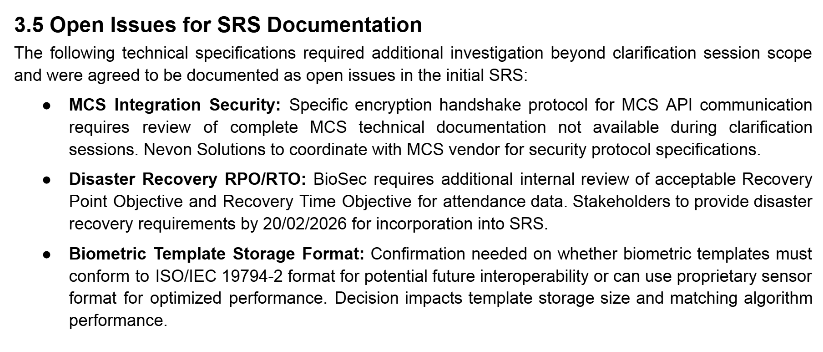
\includegraphics[width=0.9\textwidth]{evidence/analysing_open_issues.png}
\caption{Analysing Report \S3.5 — Open Issues table with deadlines}
\end{figure}

\begin{figure}[H]
\centering
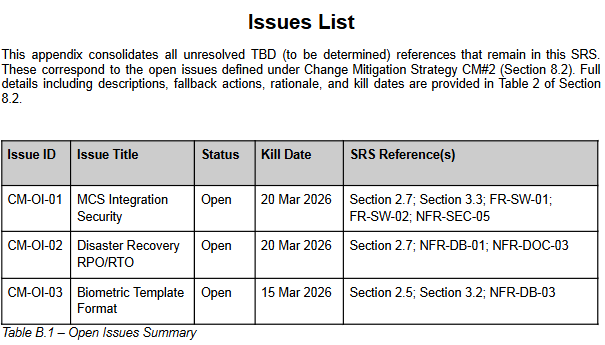
\includegraphics[width=0.9\textwidth]{evidence/srs_open_issues.png}
\caption{SRS \S2.5, \S3.3, \S6.5 — Unresolved open issues (biometric template, MCS encryption, RPO/RTO)}
\end{figure}

\vspace{0.5cm}

\subsection{Ann-002: PA-FND-002 --- SRS Sign-off Entirely Absent}
\label{ann:evidence-002}

\noindent\textbf{Related Finding:} Section~\ref{sec:findings}, PA-FND-002

\noindent\textbf{Screenshots:}

\begin{figure}[H]
\centering
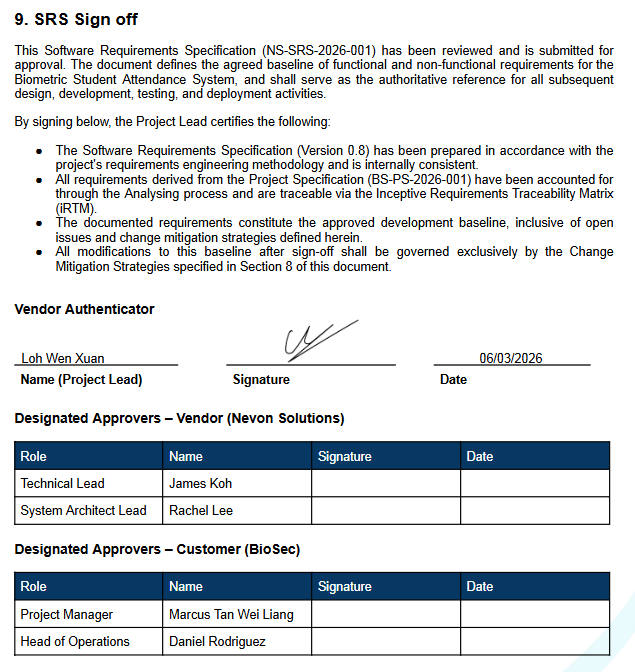
\includegraphics[width=0.9\textwidth]{evidence/srs_blank_sign_off.png}
\caption{SRS \S9 — Blank sign-off fields (all four rows empty)}
\end{figure}

\begin{figure}[H]
\centering
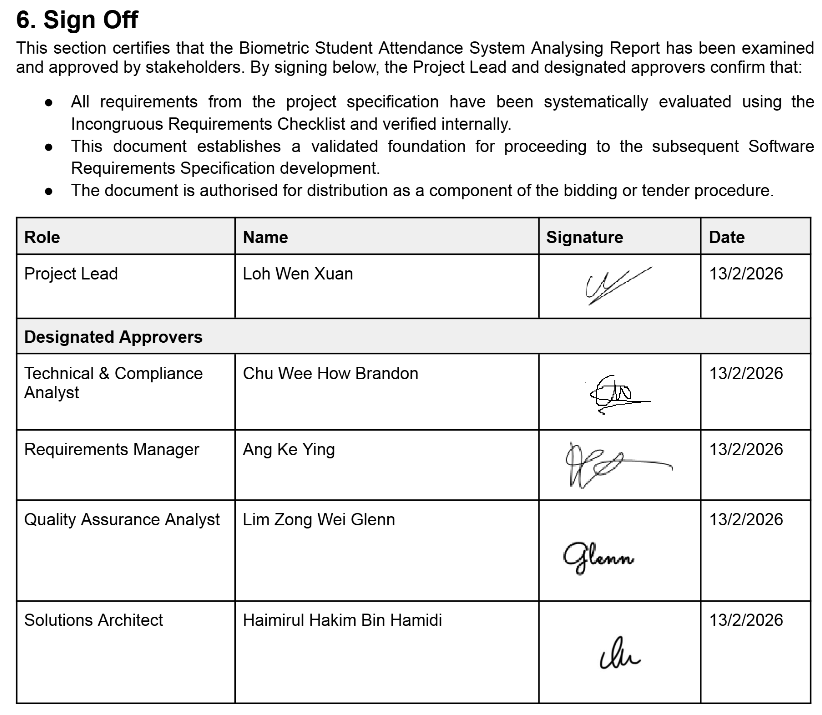
\includegraphics[width=0.9\textwidth]{evidence/analysing_report_signed.png}
\caption{Analysing Report — Correctly completed sign-off (reference)}
\end{figure}

\vspace{0.5cm}

\subsection{Ann-003: PA-FND-003 --- 2FA Scope Contradiction Not Resolved}
\label{ann:evidence-003}

\noindent\textbf{Related Finding:} Section~\ref{sec:findings}, PA-FND-003

\noindent\textbf{Screenshots:}

\begin{figure}[H]
\centering
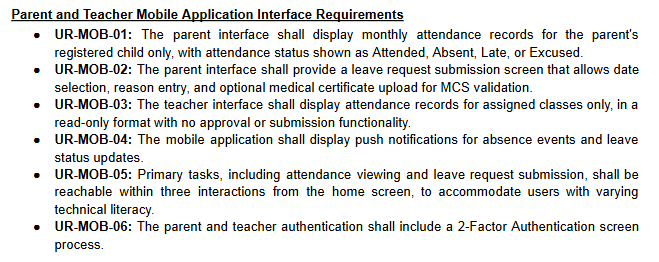
\includegraphics[width=0.9\textwidth]{evidence/srs_2fa_for_parents.png}
\caption{SRS \S3.1 UR-MOB-06 — 2FA requirement for parents and teachers}
\end{figure}

\begin{figure}[H]
\centering
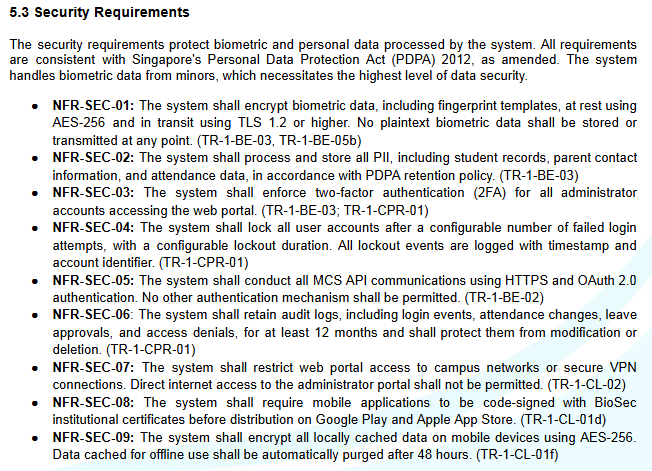
\includegraphics[width=0.9\textwidth]{evidence/srs_2fa_admins.png}
\caption{SRS \S5.3 NFR-SEC-03 — 2FA requirement for administrators only}
\end{figure}

\begin{figure}[H]
\centering
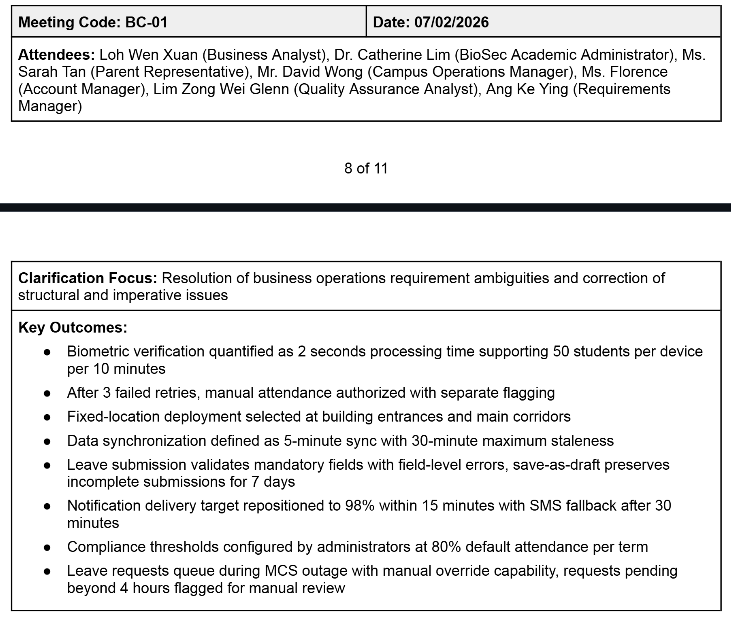
\includegraphics[width=0.9\textwidth]{evidence/BC-01.png}
\caption{Analysing Report \S3.3 — BC-01 clarification session outcomes (no 2FA resolution)}
\end{figure}

\begin{figure}[H]
\centering
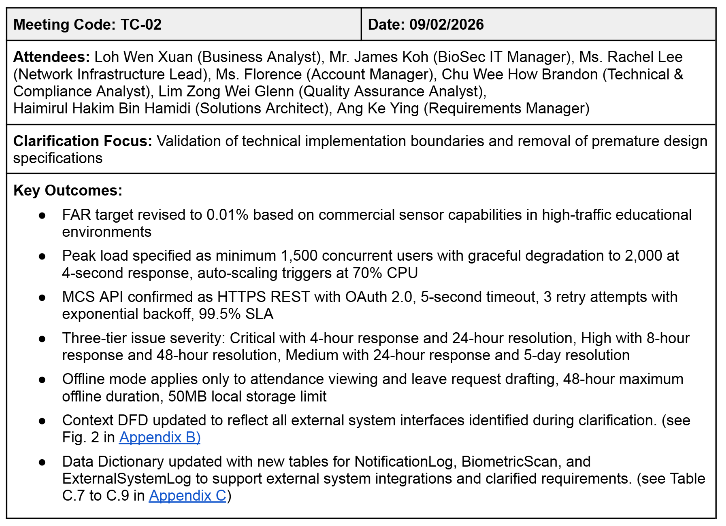
\includegraphics[width=0.9\textwidth]{evidence/TC-02.png}
\caption{Analysing Report \S3.4 — TC-02 clarification session outcomes (no 2FA resolution)}
\end{figure}

\vspace{0.5cm}

\subsection{Ann-004: PA-FND-006 --- SRS Submitted Below Final Version Threshold}
\label{ann:evidence-006}

\noindent\textbf{Related Finding:} Section~\ref{sec:findings}, PA-FND-006

\noindent\textbf{Screenshots:}

\begin{figure}[H]
\centering
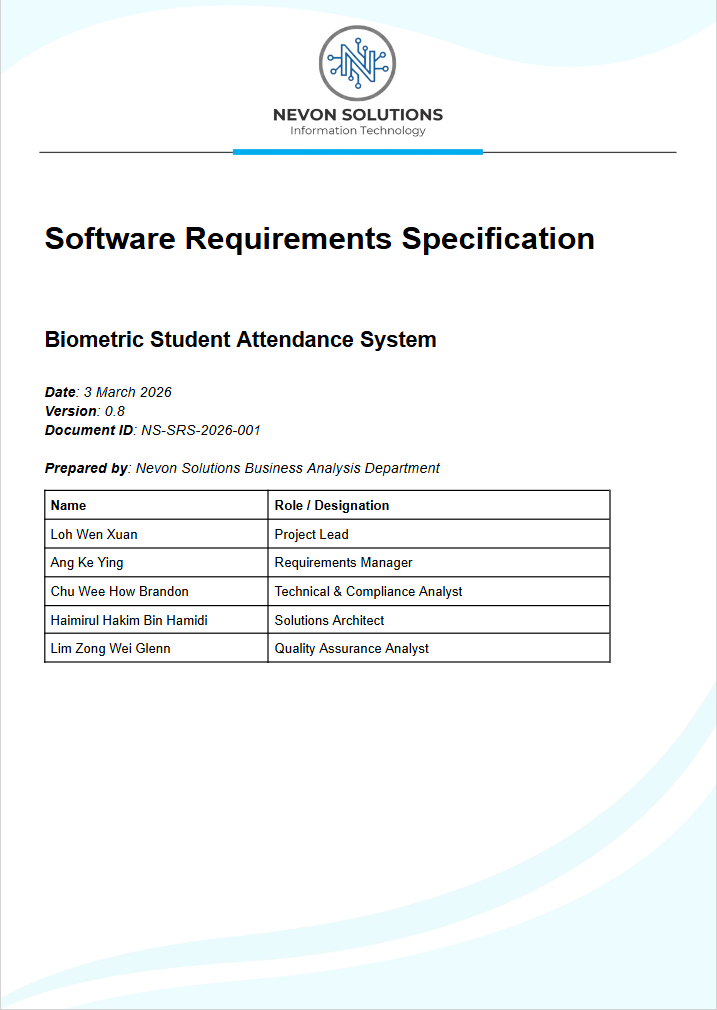
\includegraphics[width=0.9\textwidth]{evidence/srs_cover_page.png}
\caption{SRS cover page — Version 0.8, 03 March 2026}
\end{figure}

\begin{figure}[H]
\centering
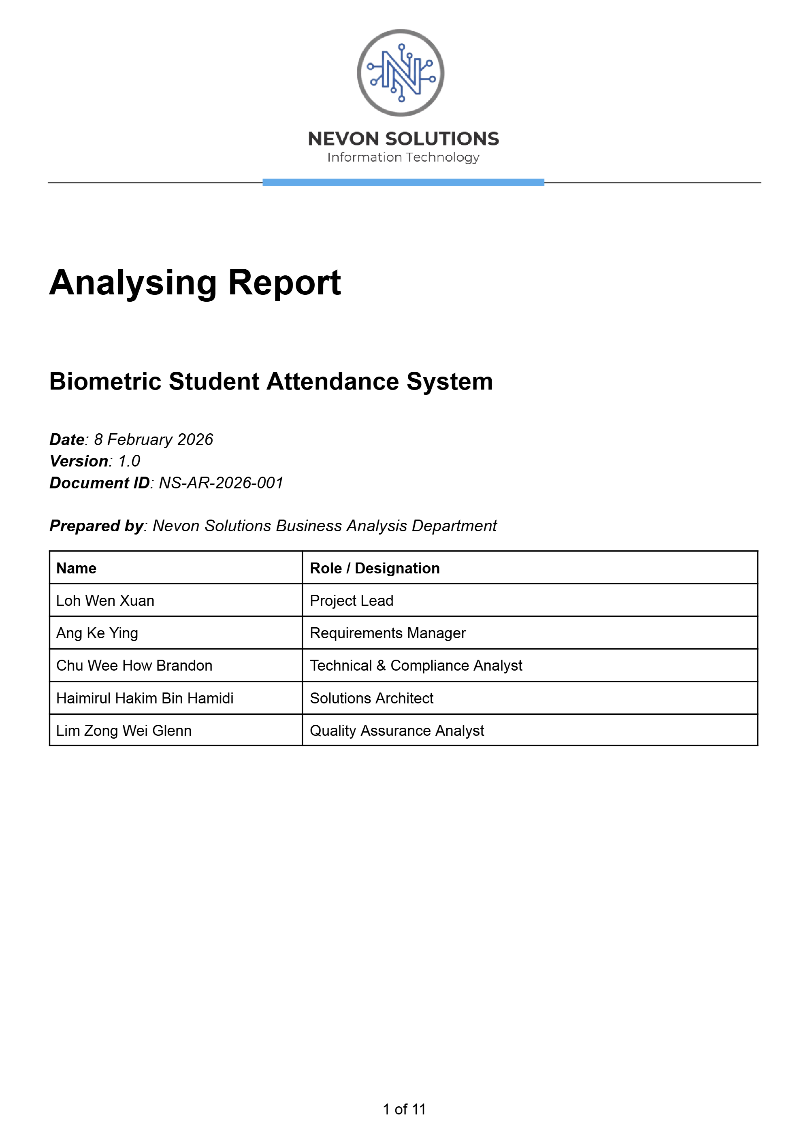
\includegraphics[width=0.9\textwidth]{evidence/analysing_report_cover_page.png}
\caption{Analysing Report cover page — Version 1.0, 08 February 2026}
\end{figure}

\vspace{1cm}
\begin{center}
    \emph{End of PA-QAR-2026-001}
\end{center}

\end{document}
